\chapter{Implementacja i porównanie}

\section{Wprowadzenie}

Opisane wcześniej algorytmy zostały zaimplementowane w języku C++ zgodnie
z przedstawionymi pseudokodami. Do implementacji struktur danych, między innymi grafów, 
wykorzystano biblioteki NetworKit oraz Koala. Kod źródłowy został dołączony
do repozytorium Koala-NetworKit na platformie \href{https://github.com/krzysztof-turowski/koala-networkit/pull/55}{GitHub}.

Wszystkie cztery algorytmy rozwiązują problem najkrótszych ścieżek pomiędzy
wszystkimi parami wierzchołków.
Trzy z nich (Seidla, USP oraz Spiry) wyznaczają odległości dokładne, natomiast
algorytm Aingwortha oblicza aproksymację addytywną: dla każdej pary
wierzchołków $(u,v)$ zwrócona wartość $\hat{\delta}(u,v)$ spełnia
$\delta(u,v) \le \hat{\delta}(u,v) \le \delta(u,v) + 2$. Algorytmy Seidla, USP oraz Aingwortha
działają na grafach nieskierowanych i nieważonych, natomiast algorytm Spiry
obsługuje grafy ważone o nieujemnych wagach krawędzi.

\section{Szczegóły implementacji}

Algorytmy zostały zaimplementowane w następujących plikach repozytorium Koala:
\begin{itemize}
    \item \texttt{include/shortest\_path/Seidel.hpp}, \texttt{cpp/shortest\_path/Seidel.cpp}
          -- algorytm Seidla (APD), oparty na mnożeniu macierzy sąsiedztwa;
    \item \texttt{include/shortest\_path/USP.hpp}, \texttt{cpp/shortest\_path/USP.cpp}
          -- algorytm USP, oparty na powtarzanym mnożeniu macierzy boolowskich
          i bitowym odzyskiwaniu odległości;
    \item \texttt{include/shortest\_path/Aingworth.hpp}, \texttt{cpp/shortest\_path/Aingworth.cpp}
          -- aproksymacyjny algorytm Aingwortha, Chekuriego, Indyka i Motwaniego (błąd $+2$);
    \item \texttt{include/shortest\_path/Spira.hpp}, \texttt{cpp/shortest\_path/Spira.cpp}
          -- algorytm Spiry dla grafów ważonych;
    \item \texttt{benchmark/benchmarkAPSP.cpp}
          -- środowisko testowe (benchmark) uruchamiające algorytmy na grafach
          z generatorów oraz porównujące ich wyniki i czasy działania.
\end{itemize}

\section{Wyniki}

\subsection{Zbiory danych}
Grafy pochodzą
z generatorów dostępnych w bibliotece NetworKit, uzupełnionych o własny generator
siatki dwuwymiarowej. Poszczególne rodziny grafów dobrano tak, aby pokrywały
różne, istotne z punktu widzenia badanych algorytmów, własności struktury grafu:
gęstość, średnicę oraz rozkład stopni. Dokładniej, użyto następujących rodzin:

\begin{description}
    \item[Graf losowy Erdősa--Rényiego $G(n,p)$.]  Model grafu losowego,
        w którym każda z $\binom{n}{2}$ możliwych krawędzi występuje niezależnie
        z prawdopodobieństwem $p$. W eksperymentach użyto wariantu \emph{rzadkiego}
        ($p = 4/n$, dającego średni stopień wierzchołka bliski $4$) oraz
        \emph{gęstego} ($p = 0{,}5$, w którym istnieje około połowy wszystkich
        możliwych krawędzi). Grafy te charakteryzują się niewielką średnicą,
        rzędu $\Theta(\log n)$, i stanowią naturalny punkt odniesienia.

    \item[Graf bezskalowy Barabásiego--Alberta.] Model grafu o tzw.
        \emph{rozkładzie potęgowym stopni} (ang. \emph{scale-free}). Graf powstaje
        przez stopniowe dodawanie wierzchołków, z których każdy łączy się z już
        istniejącymi wierzchołkami z prawdopodobieństwem proporcjonalnym do ich
        stopnia (mechanizm \emph{preferencyjnego dołączania}). W efekcie powstaje
        niewiele wierzchołków o bardzo wysokim stopniu (tzw. \emph{koncentratory},
        ang. \emph{hubs}) oraz wiele wierzchołków o niskim stopniu. Model ten
        dobrze odwzorowuje strukturę wielu sieci rzeczywistych, takich jak sieć
        WWW czy sieci społecznościowe.

    \item[Graf ,,małego świata'' Wattsa--Strogatza.] Model \emph{małego świata}
        (ang. \emph{small-world}). Powstaje z regularnego pierścienia przez losowe
        ,,przepięcie'' części krawędzi. Grafy takie łączą dwie cechy: wysoki
        \emph{współczynnik klasteryzacji} (sąsiedzi danego wierzchołka są zwykle
        również swoimi sąsiadami, co odpowiada lokalnej strukturze) oraz małą
        średnią odległość między wierzchołkami (dowolne dwa wierzchołki dzieli
        zwykle niewiele krawędzi). Model odwzorowuje wiele sieci rzeczywistych,
        w których mimo lokalnej organizacji odległości globalne pozostają krótkie.

    \item[Pierścień regularny (ang. \emph{ring lattice}).] Wierzchołki ułożone są
        na okręgu, a każdy z nich połączony jest z ustaloną liczbą najbliższych
        sąsiadów po obu stronach. Jest to graf regularny (wszystkie wierzchołki
        mają ten sam stopień) o bardzo dużej średnicy, rzędu $\Theta(n)$.
        Stanowi przypadek skrajny, obciążający algorytmy zależne od średnicy grafu.

    \item[Siatka dwuwymiarowa (ang. \emph{grid}).] Regularna siatka prostokątna,
        w której wierzchołki tworzą kratę, a krawędzie łączą sąsiadów w pionie
        i poziomie. Graf ten jest planarny, ma ograniczony stopień (co najwyżej $4$)
        oraz średnicę rzędu $\Theta(\sqrt{n})$. Jego dodatkową zaletą jest to, że
        odległości między wierzchołkami dane są jawnym wzorem (metryka miejska,
        tzw. \emph{odległość Manhattan}), co pozwala niezależnie zweryfikować
        poprawność algorytmów. Generator siatki został zaimplementowany samodzielnie,
        gdyż biblioteka NetworKit nie udostępnia go bezpośrednio.

    \item[Graf klastrowy (ang. \emph{clustered}).] Graf z wyraźną strukturą
        społecznościową: wierzchołki podzielone są na grupy (klastry), przy czym
        prawdopodobieństwo istnienia krawędzi wewnątrz grupy jest znacznie wyższe
        niż między grupami. Model odwzorowuje sieci o naturalnym podziale na
        wspólnoty.

    \item[Sieci drogowe stanów USA (\emph{roads}).]
    Zestaw obejmuje grafy planarne reprezentujące sieci dróg głównych
    wybranych stanów Stanów Zjednoczonych, pozyskane z repozytorium
    \href{https://github.com/Antoine-H/All-pairs-shortest-paths}{All-pairs-shortest-paths} (oryginalne
    dane DIMACS). Każdy wierzchołek odpowiada węzłowi drogowemu, a każda
    krawędź -- odcinkowi drogi o wadze równej jej długości.
    Grafy są planarne. Rozmiary wahają się od $n = 38$ (Hawaje, HI) do $n = 2002$
    (Pensylwania, PA). Algorytm Spiry użył oryginalnych wag krawędzi;
    pozostałe algorytmy pracowały na grafach nieważonych (wagi zignorowano).
\end{description}

Dla każdej rodziny generowano grafy o rosnącej liczbie wierzchołków $n$.
Ponieważ algorytmy Seidla oraz USP operują na gęstych macierzach o rozmiarze
$n \times n$ (algorytm USP przechowuje jednocześnie kilkadziesiąt takich macierzy),
ich zapotrzebowanie na pamięć rośnie kwadratowo z $n$; z tego powodu wszystkie klasy grafów były przetestowane na grafach z maksymalnie 5000 wierzchołów.

Ze względu na to, że badane algorytmy zakładają spójność grafu wejściowego,
z każdego wygenerowanego grafu wyodrębniano największą spójną składową,
a jej wierzchołki przenumerowywano na kolejne liczby całkowite. Dla algorytmu
Spiry, wymagającego grafu ważonego, krawędziom przypisywano wagi losowane
z rozkładu jednostajnego na przedziale $[1, 100]$. Poprawność każdej implementacji
weryfikowano przez porównanie wyznaczonych odległości z wynikami niezależnej
implementacji przeszukiwania wszerz (BFS, dla grafów nieważonych) oraz algorytmu
Dijkstry (dla grafów ważonych); w przypadku algorytmu Aingwortha sprawdzano
dodatkowo, czy zwrócone wartości mieszczą się w gwarantowanym przedziale błędu
addytywnego $+2$.

Wszystkie eksperymenty przeprowadzono na komputerze osobistym wyposażonym
w procesor Apple M1 (8 rdzeni) oraz 8 GB pamięci RAM, na systemie macOS 26.5. Kod skompilowano kompilatorem Apple Clang 17 w standardzie
C++20 z optymalizacją \texttt{-O2}.

\subsection{Empiryczna złożoność czasowa}

Dopasowując zależność $t \sim n^{\alpha}$
otrzymano wykładniki zebrane w tabeli \ref{tab:exponents}. Pokrywają się one
z przewidywaniami teoretycznymi. Algorytmy macierzowe rosną jak $n^3$
(biblioteka Eigen nie wykorzystuje szybkiego mnożenia macierzy, dlatego nie
obserwuje się wykładnika mniejszego niż $3$). Algorytmy Aingwortha i Spiry rosną
istotnie wolniej -- na grafach rzadkich, dla których zbiór wierzchołków wysokiego
stopnia jest pusty, algorytm Aingwortha degeneruje się do $n$ przeszukiwań wszerz,
stąd wykładnik bliski $2$.

\begin{table}[H]
\centering
\caption{Empiryczny wykładnik $\alpha$ w zależności $t \sim n^{\alpha}$,
         wyznaczony po odcięciu najmniejszych rozmiarów (poniżej 500 wierzchołków), oraz złożoność teoretyczna.}
\label{tab:exponents}
\begin{tabular}{lcl}
\toprule
Algorytm & $\alpha$ (empiryczny) & złożoność teoretyczna \\
\midrule
Seidel    & $2{,}9$--$3{,}2$ & $O(n^3)$ \\
USP       & $3{,}1$--$3{,}2$ & $O(n^3 \log n)$ \\
Aingworth & $2{,}1$--$2{,}4$ & $O(n^{2{,}5}\sqrt{\log n})$ \\
Spira     & $2{,}0$--$2{,}3$ & $O(n^2 \log n)$  \\
\bottomrule
\end{tabular}
\end{table}

\subsection{Porównanie czasów działania}

Rysunek \ref{fig:apsp-runtime} przedstawia czasy działania dla czterech rodzin
grafów w funkcji liczby wierzchołków $n$ (skala logarytmiczna na obu osiach).
Najważniejsze obserwacje, dla $n \approx 5000$, są następujące:

\begin{itemize}
    \item Algorytm \textbf{USP} jest bezwzględnie najwolniejszy, a jego czas jest
        niemal \emph{niezależny od rodziny grafu} (około $295$ s dla każdej klasy)
        -- koszt zależy wyłącznie od $n$, a nie od liczby krawędzi. Jest on
        $5$--$70$ razy wolniejszy od algorytmu Seidla i $425$--$1034$ razy wolniejszy
        od algorytmu Aingwortha. Mimo że asymptotycznie zbliżony do algorytmu Seidla,
        ma wielokrotnie większą stałą (odzyskiwanie kolejnych bitów odległości
        wymaga kilkudziesięciu mnożeń macierzy zamiast kilku).

    \item Algorytm \textbf{Aingwortha} jest najszybszy w każdej klasie
        ($0{,}27$--$0{,}70$ s przy $n \approx 5000$). Na grafach gęstych bije nawet
        naiwne wyznaczanie APSP za pomocą $n$ przeszukiwań wszerz: $472$ ms wobec
        $53$ s, czyli około $100$-krotnie szybciej.

    \item Algorytm \textbf{Seidla} wyprzedza pozostałe algorytmy dokładne
        \emph{tylko na grafach gęstych} ($4{,}2$ s wobec $22{,}8$ s dla algorytmu
        Spiry), ponieważ jego koszt nie zależy od liczby krawędzi. Na grafach
        rzadkich zależność się odwraca: przy $n=5000$ algorytm Seidla ($19{,}9$ s)
        jest wolniejszy od algorytmu Spiry ($12{,}2$ s), a na siatce dwuwymiarowej,
        o dużej średnicy, różnica jest znaczna ($55{,}4$ s wobec $5{,}7$ s). Wynika
        to z dwóch efektów: algorytm Spiry korzysta z rzadkości grafu, natomiast
        algorytm Seidla wykonuje tym więcej poziomów rekursji, im większa jest
        średnica grafu.
\end{itemize}

\begin{table}[H]
\centering
\small
\setlength{\tabcolsep}{5pt}
\renewcommand{\arraystretch}{1.2}
\begin{tabular}{lrrrrrrr}
\toprule
\textbf{Graf} & $n$ & $m$ & Seidel [ms] & USP [ms] & Aingworth [ms] & Spira [ms]  \\
\midrule
HI & 38 & 43 & 0.07 & 0.18 & 0.04 & 0.10 \\
DE & 148 & 216 & 1.61 & 5.27 & 0.29 & 1.74 \\
NH & 197 & 275 & 3.18 & 13.01 & 0.59 & 4.42 \\
ME & 221 & 318 & 5.03 & 16.92 & 0.73 & 5.68 \\
AZ & 225 & 308 & 4.85 & 19.11 & 0.76 & 6.13 \\
MA & 381 & 571 & 23.32 & 98.78 & 2.04 & 20.08\\
MN & 798 & 1222 & 188.7 & 942.3 & 9.11 & 102.7 \\
VA & 886 & 1340 & 292.7 & 1225.5 & 10.26 & 119.7 \\
CA & 935 & 1373 & 354.3 & 1499.0 & 11.81 & 125.8 \\
NC & 948 & 1432 & 390.9 & 1579.2 & 13.51 & 139.3 \\
OH & 998 & 1620 & 367.6 & 1763.4 & 15.35 & 176.7 \\
IL & 1299 & 1997 & 811.4 & 4406.2 & 25.55 & 292.8 \\
FL & 1317 & 1894 & 954.3 & 4523.4 & 20.93 & 246.4 \\
NY & 1437 & 2271 & 1283.1 & 5939.0 & 26.06 & 337.0 \\
GA & 1557 & 2508 & 1575.6 & 7689.6 & 37.72 & 439.8 \\
TX & 1755 & 2758 & 2260.7 & 10853 & 46.12 & 628.1  \\
PA & 2002 & 2898 & 3243.7 & 15904 & 64.92 & 638.0  \\
\bottomrule
\end{tabular}
\caption{Czasy działania algorytmów APSP na grafach z zestawu roads.}
\label{tab:real-roads}
\end{table}

Tabela \ref{tab:real-roads} prezentuje wyniki dla sieci drogowych
$17$ stanów USA, posortowanych rosnąco według liczby wierzchołków $n$.

Każdy z przebiegów algorytmu Aingwortha wykazał zerowy błąd. Wynika to ze struktury grafów.
Algorytm Aingwortha wyznacza zbiór dominujący oparty na wierzchołkach
wysokiego stopnia. Badane grafy były rzadkie, a stopień każdego
wierzchołka był ograniczony,
więc zbiór dominujący jest pusty i algorytm degeneruje się do $n$
przeszukiwań wszerz -- zachowując się identycznie jak naiwna metoda BFS.

Ranking czasów jest spójny z wynikami dla pozostałych grafów rzadkich:
najszybszy jest Aingworth ($0{,}04$--$65$ ms), następnie Spira
($0{,}10$--$638$ ms), dalej Seidel ($0{,}07$--$3244$ ms),
a algorytm USP jest zdecydowanie najwolniejszy ($0{,}18$--$15904$ ms).

Wzrost czasów działania wraz z $n$ jest zgodny z przewidywaniami
teoretycznymi. Algorytm Seidla -- mimo teoretycznej złożoności
$O(n^\omega \log n)$ -- w praktyce wypada gorzej od Spiry dla grafów
rzadkich, gdyż opiera się na mnożeniu gęstych macierzy, co jest
nieefektywne gdy $m \ll n^2$.

Ranking algorytmów zależy zatem od struktury grafu: na grafach gęstych o małej
średnicy przewagę ma podejście macierzowe (Seidel), a na grafach rzadkich --
podejście oparte na pojedynczych źródłach (Spira). Algorytm Aingwortha, kosztem
dopuszczenia błędu addytywnego $+2$, jest najszybszy niezależnie od klasy grafu.

\begin{figure}[t]
    \centering
    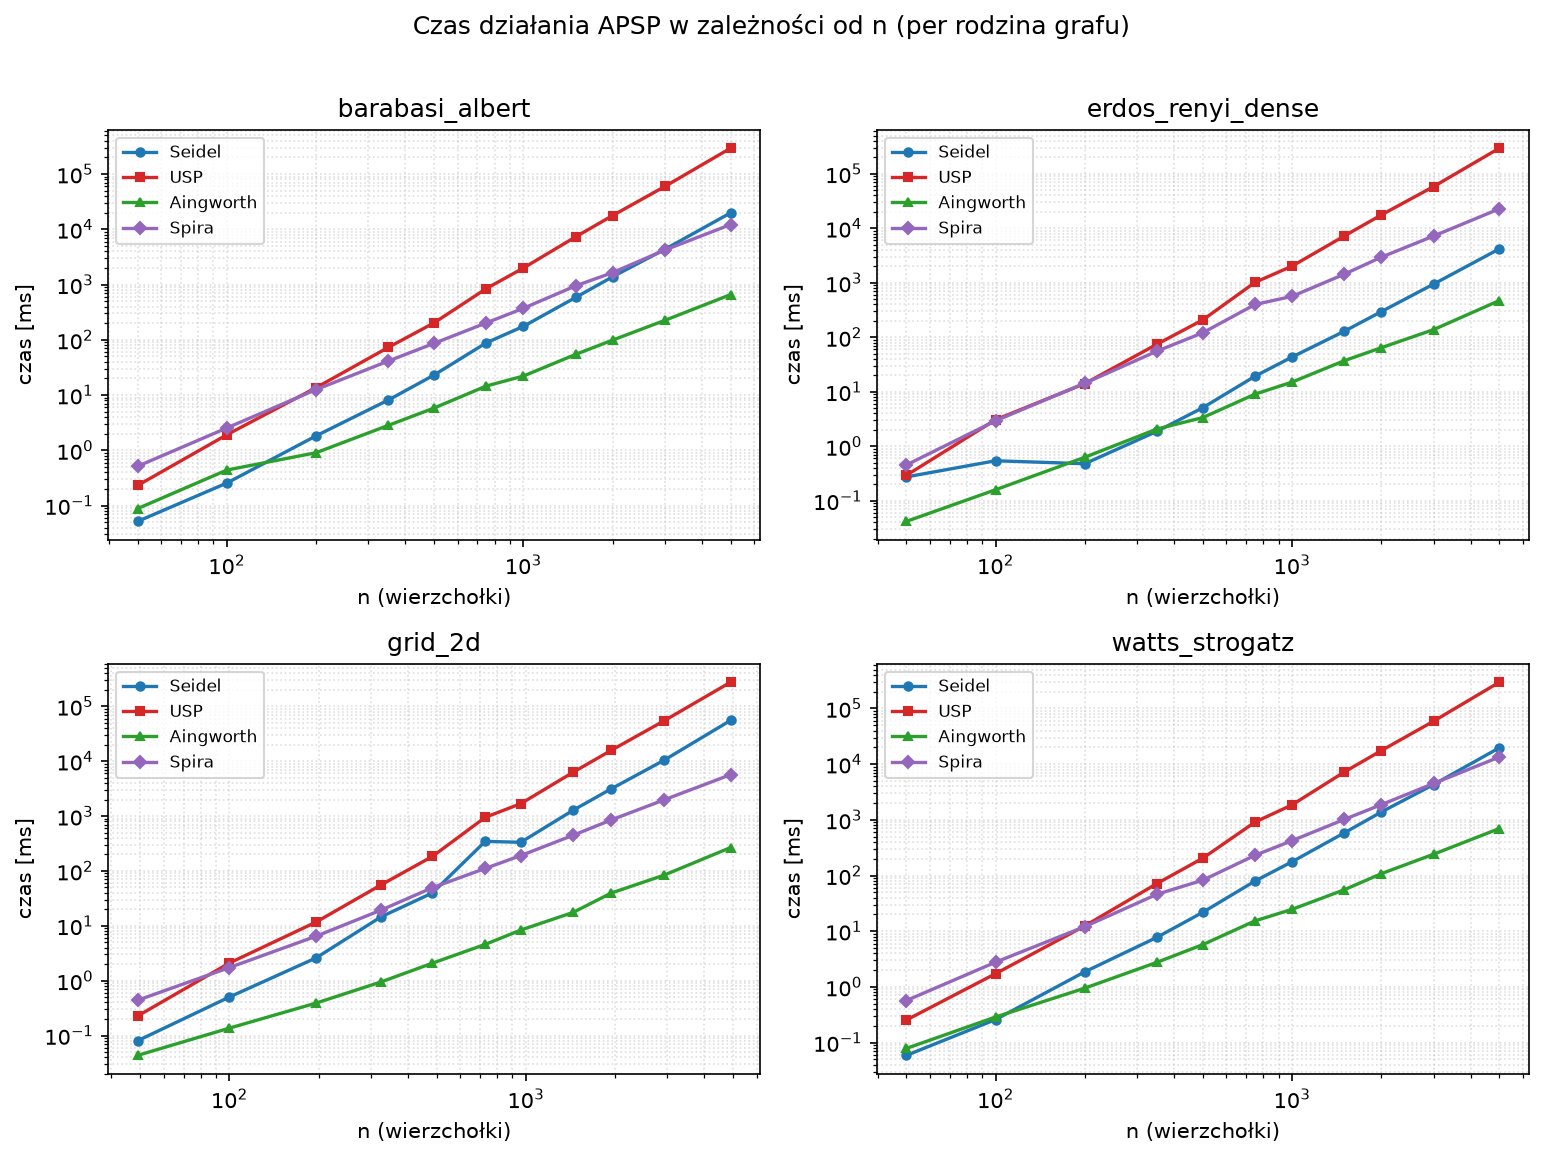
\includegraphics[width=\linewidth]{runtime_by_generator.png}
    \caption{Czas działania algorytmów APSP w zależności od liczby wierzchołków $n$
             dla czterech rodzin grafów (skala logarytmiczna na obu osiach).
             Wszystkie cztery algorytmy uruchomiono dla rozmiarów do $n=5000$.}
    \label{fig:apsp-runtime}
\end{figure}

\subsection{Dokładność aproksymacji Aingwortha}

Choć algorytm gwarantuje błąd co najwyżej $+2$, w praktyce błąd ten pojawiał się
jedynie dla części grafów:

\begin{itemize}
    \item graf gęsty Erdősa--Rényiego -- błąd $+2$ wystąpił dla każdego
        badanego rozmiaru;
    \item graf bezskalowy Barabásiego--Alberta -- błąd $+2$ jedynie dla
        najmniejszego grafu ($n=50$);
    \item graf małego świata oraz siatka dwuwymiarowa -- wynik był
        zawsze dokładny.
\end{itemize}

Błąd addytywny koreluje z gęstością i małą średnicą grafu: im krótsze odległości
i im więcej par wierzchołków znajduje się w tej samej odległości, tym częściej
zaokrąglenie wewnątrz algorytmu prowadzi do przeszacowania. Na grafach rzadkich
o dużej średnicy algorytm Aingwortha zachowywał się w przeprowadzonych testach jak
metoda dokładna.

\subsection{Uwagi dotyczące zużycia pamięci}

Algorytmy Seidla i USP operują na gęstych macierzach $n \times n$. Algorytm USP
przechowuje ich kilkadziesiąt jednocześnie, co teoretycznie odpowiada około $8$ GB
pamięci dla $n=5000$. W praktyce maksymalne zużycie pamięci całego programu wyniosło około $1{,}3$ GB dla wszystkich instancji testowych
oprócz grafów internetowych $AS$ z repozytorium \cite{antoine2025apsp},
które zawierają około $15\,000$ wierzchołków. Dla tych grafów zużycie
pamięci przekroczyło $18$ GB, co uniemożliwiło przeprowadzenie testów
na dostępnym sprzęcie.

\subsection{Wnioski}

Zebrane wyniki prowadzą do następujących wniosków praktycznych:
\begin{enumerate}
    \item Algorytm \textbf{USP} ma przede wszystkim znaczenie teoretyczne -- jego
        stała jest na tyle duża, że pozostaje niepraktyczny nawet dla umiarkowanych
        wartości $n$. 
    \item Algorytm \textbf{Seidla} opłaca się na grafach gęstych o małej średnicy;
        na grafach rzadkich lub o dużej średnicy ustępuje prostszemu algorytmowi
        \textbf{Spiry}.
    \item Algorytm \textbf{Aingwortha} był najszybszy we wszystkich testowanych
        klasach grafów i często dokładny; stanowi atrakcyjny wybór, gdy dopuszczalny
        jest niewielki błąd addytywny.
\end{enumerate}


\newpage